\chapter{A Evasão nas Instituições de Ensino Superior} \label{2title}

A evasão nas Instituições de Ensino Superior é um problema antigo, mas pouco explorado no meio educacional. Os cursos de Ciências Exatas, tais como Matemática, Física e Ciência da Computação, geralmente apresentam taxas de alunos formados inferiores se comparadas às outras áreas de conhecimento \citep{censo2013}. Neste capítulo, será abordado o conceito, fatores e situações que justifiquem as taxas de evasão na área de Computação, objeto de estudo desta pesquisa. A Seção \ref{2title1} retrata o panorama da Educação Superior conforme o Censo da Educação Superior de 2013. A Seção \ref{2title2} aborda os conceitos de evasão, exclusão e mobilidade, além das implicações que a evasão acarreta ao aluno e ao sistema de ensino. A Seção \ref{2title3} aponta os principais motivos apontados para justificar a evasão dos alunos dos cursos de graduação, incluindo análises de evasão no âmbito da Universidade de Brasília. A Seção \ref{2title4} apresenta estudos relacionados à evasão nos cursos de Computação no Brasil. A Seção \ref{2title5} apresenta estudos realizados sobre evasão nos cursos de Computação da Universidade de Brasília, e a Seção \ref{2title6} apresenta a análise dos resultados observados nas  Seções \ref{2title4} e \ref{2title5}. 

\section{O Cenário da Educação Superior no Brasil} \label{2title1}

Anualmente, o Censo da Educação Superior, realizado pelo Instituto Nacional de Estudos e Pesquisas Educacionais Anísio Teixeira (INEP)~\footnote{\url{http://portal.inep.gov.br}}, vinculado ao Ministério da Educação~\footnote{\url{http://www.mec.gov.br}} fornece dados que permitem analisar a Educação Superior no Brasil. O Censo Escolar consiste na levantamento e análise de dados estatísticos educacionais do cenário nacional.

De acordo com os resultados obtidos pelo Censo da Educação Superior de 2013 \citep{censo_site}, no Brasil haviam 32.049 cursos de graduação, sendo 30.791 presenciais e 1.258 a distância. Também foram contabilizadas 2.391 Instituições de Ensino Superior, sendo 301 públicas e 2.090 particulares, conforme mostrado na Tabela \ref{instituiçoes}. As Instituições particulares correspondem a 87,41\% das Instituições de Ensino Superior no Brasil, e deste total, 89,76\% correspondem à faculdades privadas.

\begin{table}[!h]
	\caption{Número de Instituições de Ensino Superior no Brasil em 2013.} 	\label{instituiçoes}
	\centering
	\begin{tabular}{C{4cm}|C{3cm}C{3cm}}
		\hline
		Categoria & \multicolumn{2}{c}{Quantidade}\\
		\hline
		& Pública & Privada\\ \hline
		Universidade & 111 & 84\\
		Centro Universitário & 10 & 130\\
		Faculdade & 140 & 1.876\\
		IF e Cefet~\footnote{IF: Institutos Federais; Cefet: Centro Federal de Educação Tecnológica.} & 40 & -\\
		\hline
	\end{tabular}
\end{table}

Em 2013, foram registrados 7,3 milhões de alunos matriculados no ensino superior, representando um crescimento de 3,8\% em relação ao ano de 2012. Entre o ano de 2012 e 2013, foi verificado um crescimento de 4,5\% na rede privada e 1,9\% na rede \citep{censo2013}. Em 2013, as universidades atendiam 53,4\% e as faculdades 29,2\% das matrículas. Em relação ao ano de 2003, foi verificado um crescimento de 76,4\% no número de matrículas, conforme apresentado na Figura \ref{graficoCenso}. 

\begin{figure}[!h]
	\centering
	{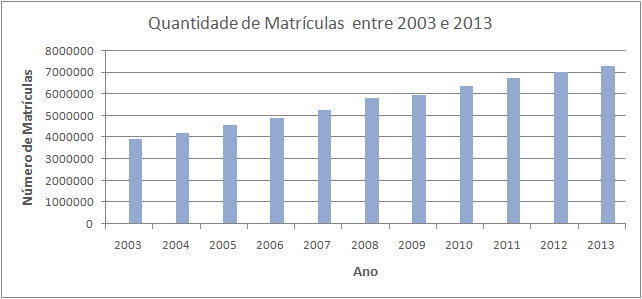
\includegraphics[width=13cm, height=6cm]{images/censo_matriculas}}
	\caption {Quantidade de matrículas registradas pelo Censo da Educação Superior entre o ano de 2003 e 2013.}
	\label{graficoCenso}
\end{figure}

A Figura \ref{distribuicao} apresenta a distribuição das matrículas por tipo de Instituição de Ensino Superior. As universidades eram responsáveis por 70,8\%, os centros universitários por 25,2\%, as faculdades por 3,2\%, e os institutos federais e centros federais de educação tecnológica por 0,8\% das matrículas efetivas em 2013. As Instituições privadas eram responsáveis por 86,6\% e as Instituições públicas 13,4\% das matrículas.

\begin{figure}[!h]
	\centering
	{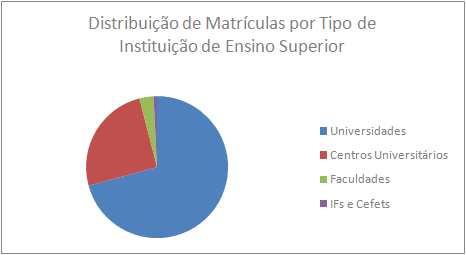
\includegraphics[width=12cm, height=6cm]{images/distribuicao}}
	\caption {Distribuição de Matrículas por tipo de Instituição de Ensino Superior. As universidades eram responsáveis pelo maior percentual de matrículas efetivas em 2013.}
	\label{distribuicao}
\end{figure}

Dos 1.951.354 alunos ingressantes em 2013, 56,44\% são do sexo feminino e 45,34\% do sexo masculino. Das 6.152.405 matrículas registradas, 55,52\% são do sexo feminino e 44,48\% do sexo masculino. Dos 829.938 alunos concluintes, 59,24\% são do sexo feminino e 40,76\% do sexo masculino. Analisando o quantitativo de matrículas efetivas, alunos formados e concluintes por tipo de Instituição, as Instituições de Ensino Superior privadas são responsáveis por atender uma maior demanda de alunos, conforme apresentado na Tabela \ref{atendimento}. Outro dado revelado pelo Censo é que as Instituições de Ensino Superior públicas abrangem aproximadamente 28,9\% das matrículas efetivas, e as Instituições de Ensino Superior privadas aproximadamente 71,1\%.

\begin{table}[!h]
	\caption{Número de alunos atendidos pelas Instituições de Ensino Superior públicas e privadas.} 	\label{atendimento}
	\centering
	\begin{tabular}{C{4cm}|C{3cm}C{3cm}}
		\hline
		Categoria & \multicolumn{2}{c}{Quantidade}\\
		\hline
		& Pública & Privada\\ \hline
		Alunos Ingressantes & 456.864 & 1.494.490\\
		Matrículas Efetivas & 1.777.974 & 4.374.431\\
		Alunos Concluintes & 206.261 & 623.677\\ \hline
	\end{tabular}
\end{table}

A Tabela \ref{areas} mostra o percentual de matrículas, ingressantes e concluintes por área geral de curso. A área de Ciências Sociais, Negócios e Direito apresentou o maior percentual de matrículas, ingressantes e concluintes em 2013, seguida da área de Educação. Nas áreas de Engenharia, Produção e Construção, Ciência, Matemática e Computação, e Agricultura e Veterinária, o percentual de concluintes é menor se comparado ao percentual de matriculados e ingressos.

\begin{table}[!h]
	\caption{Percentual de Matrículas, Ingressantes e Concluintes por Área de Atuação em 2013.} 	\label{areas}
	\centering
	\begin{tabular}{C{7cm}|C{2cm}C{2,5cm}C{2,5cm}}
		\hline
		Área de Atuação & \multicolumn{3}{c}{Percentual (\%)}\\
		\hline
		& Matrículas & Ingressantes & Concluintes \\ \hline
		Ciências Sociais, Negócios e Direito & 40,6 & 41,5 & 44,3\\
		Educação & 18,8 & 17,2 & 20,3\\
		Saúde e Bem Estar Social & 13,5 & 12,5 & 14,1\\
		Engenharia, Produção e Construção & 14 & 14,8 & 8,2\\
		Ciência, Matemática e Computação & 6,1 & 6,5 & 5,6\\
		Agricultura e Veterinária & 2,4 & 2,1 & 1,9\\
		Humanidades e Artes & 2,2 & 2,4 & 2,7\\
		Serviços & 2,3 & 3,1 & 2,9\\
		\hline
	\end{tabular}
\end{table}

 
Em contraste ao crescimento do número de ingressantes, os resultados também apontaram uma redução na quantidade de alunos formados nas Instituições de Ensino Superior brasileiras. Em 2013, foram contabilizados 991.010 alunos formandos nos cursos de graduação em todo o Brasil, 5,7\% a menos em relação ao ano de 2012, que contabilizou 1.050.413 alunos formandos \citep{censo2012}. Analisando a taxa de concluintes por tipo de Instituição de Ensino Superior, foi verificada uma redução aproximada de 6,7\% nas Instituições privadas e de 3,5\% nas Instituições públicas em relação ao ano de 2012. 

Apesar do crescimento e expansão do acesso ao Ensino Superior nos últimos anos no Brasil, percebe-se ainda que o número de concluintes é inferior ao número de matrículas efetivas. Tomando como exemplo a área de Ciências, Matemática e Computação, apenas 12,5\% dos alunos foram identificados como concluintes em 2013, se comparado ao total matrículas efetivas para a área no mesmo período. Conforme destacado por \citet{tigrinho2008}, apenas o ingresso do aluno nos cursos de graduação não é suficiente para garantir a permanência e conclusão do ensino superior. 

A fim de identificar e compreender as causas de desistência ou abandono escolar nos cursos de graduação, estudos e pesquisas a respeito da evasão escolar vêm crescendo e ganhando destaque no meio educacional. \citet{lobo2011} e \citet{dias2010} destacam a evasão como uma dos principais problemas em qualquer nível de ensino, que aflige as Instituições de Ensino em geral, sejam elas públicas ou particulares.
 

\section{O Conceito de Evasão e sua Implicação na Gestão das Instituições de Ensino Superior} \label{2title2}

A evasão escolar tem se tornado um  objeto de estudo nos diferentes níveis da educação, desde a educação básica até o ensino superior. Embora no Brasil o número de pesquisas relacionadas ao assunto tenha crescido nos últimos anos, \citet{lobo2011} afirma que ainda não existem estudos suficientes que abordem a evasão no cenário nacional, sendo a maioria das análises limitadas a casos isolados (limitados a uma Instituição de Ensino Superior ou a um docente), se comparados aos países desenvolvidos. No sentido geral, a evasão escolar pode ser caracterizada pelo abandono ou interrupção dos estudos, de forma voluntária ou involuntária, que pode ser influenciado por uma conjunção de fatores internos ou externos ao indivíduo. \citet{gaioso2005} interpreta a evasão escolar como a interrupção dos estudos, sem a sua conclusão. 

O conceito de evasão, por sua vez, pode ser confundido com o conceito de exclusão e mobilidade. Para \citet[p. 13]{bueno1993}, a evasão é caracterizada pelo desligamento voluntário do aluno, por sua própria vontade e responsabilidade, enquanto que a exclusão \textit{"implica na admissão de uma responsabilidade da escola e de tudo que a cerca por não ter mecanismos de aproveitamento e direcionamento do adolescente que se apresenta para uma formação profissionalizante."} Do mesmo modo, \citet{ristoff1997} traz o paralelo entre os conceitos de evasão e mobilidade, onde a evasão corresponde ao abandono dos estudos, enquanto a mobilidade caracteriza-se pela mudança de curso, como uma tentativa de se encontrar êxito ou felicidade sobre suas reais possibilidades e potencialidades.

A evasão pode estar relacionada a fatores institucionais, pessoais e externos. E pode consistir em evasão de um curso, de uma universidade ou do sistema de ensino superior. Nesse sentido, a Comissão Especial de Estudos sobre Evasão \citep{mec_1997} define o processo de evasão em três níveis: evasão do curso, evasão da instituição e evasão do sistema.

A evasão do curso é aquela que o aluno deixa o curso por alguma razão, podendo permanecer na mesma Universidade, ou mudar para outro curso de outra Instituição de Ensino Superior ou abandonar os estudos universitários. De acordo com o \citet{mec_1997}, esse tipo de evasão pode ocorrer por abandono, mudança de curso, desistência ou exclusão por norma institucional. Em qualquer dos casos, o aluno é desligado do curso, o que consiste em uma evasão, e essa deverá ser estudada para que outras perdas de mesma natureza sejam evitadas. A evasão da instituição é aquela que ocorre quando um estudante vai para uma outra Instituição de Ensino Superior, o que ocorre na maior parte das vezes por um problema de gestão e de insatisfação do estudante com o ambiente educacional. E existe também a evasão do sistema, onde o aluno interrompe o ensino superior, seja temporariamente ou definitivamente. Esse tipo de evasão é que demanda mais atenção por parte do Governo, pois pode implicar em mudanças na políticas públicas de educação, desde questões institucionais, acadêmicas ou até mesmo individuais. A evasão escolar não é problema restrito somente ao Brasil. Segundo \citet{silvafilho2007}, a evasão no ensino superior é uma problemática internacional, que exerce impacto nos resultados sobre os sistemas educacionais. 

Um apontamento interessante  destacado por \citet{silvafilho2007} é a ausência de programas que visem a permanência do aluno junto à instituição de ensino. Nas instituições privadas, um grande esforço de propaganda e \textit{marketing} é empregado para atrair novos alunos, porém tal esforço não é destinado à manutenção dos alunos já matriculados. Para \citet[p. 642]{silvafilho2007}, \textit{"as perdas de estudantes que iniciam mas não terminam seus cursos são desperdícios sociais, acadêmicos e econômicos"}, o que acarreta na perda de recursos e receitas, pois tornam-se investimentos sem retorno, sejam estes financeiros ou não. Segundo o pesquisador Oscar Hipólito, do Instituto Lobo para o Desenvolvimento da Educação, da Ciência e da Tecnologia~\footnote{Publicação disponível em \url{http://g1.globo.com/educacao/noticia/2011/02/pais-perde-r-9-bilhoes-com-evasao-no-ensino-superior-diz-pesquisador.html}}, as perdas financeiras com evasão no ensino superior em 2009 alcançou a marca de 9 bilhões de reais.

\citet{tigrinho2008} também caracteriza as perdas ocorridas no processo de evasão escolar. Para o autor, há perdas de caráter econômico, tanto para o aluno quanto para a Instituição de Ensino. As instituições podem ser afetadas pela perda de prestígio e impactos financeiros, principalmente as Instituições de Ensino Superior privadas. \citet{lobo2011} também salienta os possíveis prejuízos para as Instituições de Ensino Superior privadas. Uma vez que os cursos são planejados tomando por base a quantidade de alunos pagantes, a geração de vagas ociosas pode acarretar em problemas gerenciais e afetar a viabilidade dos cursos e das próprias Instituições, visto que a redução das receitas podem comprometer os planos administrativo-financeiro e acadêmico.

\citet{braga2003} demonstram que, ao estudar a evasão, outros aspectos relacionados à Instituições de Ensino Superior também devem ser considerados, tais como a avaliação da estruturas curriculares dos cursos, participação dos docentes e discentes na elaboração das propostas curriculares, metodologias pedagógicas empregadas, cultura organizacional do ambiente escolar e a figura do docente em sala de aula. Conforme \citet{baggi_lopes2010}, uma análise abrangente do âmbito da instituição é capaz de revelar informações que podem ser úteis para a resolução de problemáticas enfrentadas, na revisão de processos utilizados e no aprimoramento do ensino. Portanto, a evasão não deve ser atribuída somente ao aluno, passando a ser também uma reflexão sobre a própria estrutura geral da Instituição, o que envolve um processo de análise qualitativa e quantitativa como um todo. \citet[p. 59]{favero2013}  \textit{apud} \citet{lobo2011} salientam que a questão da evasão deve ser trabalhada em conjunto com todos os membros da Instituição de Ensino Superior, num esforço coletivo entre os profissionais da área acadêmica e administrativo-financeira, de modo que as ações desenvolvidas de combate à evasão não sejam vistas \textit{"apenas como uma gestão de marketing ou atendimento, mas fazer parte das ações estratégicas, com planejamento, execução, acompanhamento e avaliação".} Conforme o \citet[p. 19]{mec_1997}, 
\begin{quotation}
\textit{"Compreender a evasão como um processo implica superar a postura economicista, derivada de visão essencialmente utilitarista da formação universitária que, se levada a extremos, conduziria, por exemplo, à extinção de alguns cursos que são hoje mantidos quase que exclusivamente pelas universidades públicas. Logo, os índices de diplomação, retenção e evasão devem ser examinados em conjunto, não como um fim em si mesmos, ou apenas com objetivos "rankeadores", mas sim como dados que possam contribuir tanto à identificação dos problemas a eles relacionados, como à adoção de medidas pedagógicas e institucionais capazes de solucioná-los".}
\end{quotation}

\section{Motivos para Evasão} \label{2title3}

A evasão é um problema complexo, que pode ser resultante de uma conjunção de vários fatores que pesam na decisão do aluno de permanecer ou não no curso \cite{tigrinho2008}. As causas para a desistência são variadas, mas o essencial é que o aluno não pare de estudar por falta de condições. Alguns fatores são citados como os mais recorrentes:

\begin{itemize} 
\item \textit{Repetência:} O baixo rendimento e a reprovação em disciplinas consideradas difíceis influenciam na decisão de continuar ou não os estudos, principalmente se esta ocorre nos semestres iniciais. Essa é considerada a causa principal de evasão. Um fator que também pode contribuir para repetência, conforme destaca \citet{tigrinho2008}, é a forma de avaliação utilizada pela Instituição de Ensino;

\item\textit{ Baixa eficiência durante o Ensino Médio:} Esse item relaciona-se diretamente com a repetência, pois o aluno que passa na seleção do vestibular mas não possui uma base de conhecimento consolidada provavelmente encontrará dificuldades de adaptação e não conseguirá realizar um bom acompanhamento durante o curso;

\item \textit{Falta de conhecimento acerca dos cursos e escolha precoce da especialidade funcional:} São mais de 150 opções de cursos superiores e, a cada dia, surgem novas opções de carreiras e de oportunidades de trabalho. A escolha da profissão geralmente acontece muito cedo, geralmente logo após o término do Ensino Médio. A indecisão é normal nessa fase e muitas vezes não se investiga as opções de cursos pelos melhores critérios. A escolha pode advir de uma expectativa irreal que é frustrada após a entrada do estudante na Universidade. A falta de informações sobre a profissão e o curso em que os alunos ingressam leva muitos à evasão. Ao perceberem que agiram movidos por ideias infundadas a respeito da instituição ou da profissão escolhida, se decepcionam com o curso superior e a Instituição de Ensino. Logo passam a considerar a possibilidade de desistência;

\item \textit{Mudança de curso:} Há vários fatores que podem levar o estudante a mudar de curso, como a não identificação com o curso atual, dificuldades nas disciplinas, mudança de área em que se deseja atuar, entre outros. A mudança pode ocorrer tanto na mesma Instituição de Ensino (no caso ocorre somente a mudança de curso), como para outras Instituições de Ensino Superior (neste caso, pode ser que o aluno queira continuar no mesmo curso, mas em outra Instituição). Em muitos casos, há a possibilidade de aproveitamento de disciplinas equivalentes, o que facilita tal mobilidade entre cursos;

\item \textit{Desprestígio da profissão:} Conforme destacado por Tigrinho (2008), esse fator está muitas vezes está relacionado à visão que foi e é construída sobre o curso e a área de atuação. Áreas como Medicina, Engenharia e Direito, por exemplo, pressupõem para muitas pessoas prestígio social, salários acima da média e maiores e facilitadas chances de empregabilidade. Por outro lado, percebe-se o oposto em cursos como as Licenciaturas, marcadas por sobrecarga na jornada de trabalho e salários reduzidos se comparados à outras áreas de atuação, o que contribui para que a falta de prestígio e visibilidade da profissão diante do mercado de trabalho;

\item \textit{Restrições nos financiamentos estudantis e dificuldades financeiras:} Mesmo com a existência e expansão de programas que visem contribuir com os custos de um curso superior, tais como o Fundo de Financiamento Estudantil (FIES) e o Programa Universidade para Todos (PROUNI), ainda não é suficiente para atender todos os alunos que não possuem meios financeiros para se manter na Universidade;

\item \textit{Horário do trabalho:} Muitas pessoas trabalham que têm a necessidade de trabalhar e estudar ao mesmo tempo podem encontrar dificuldades quanto à conciliação de horários. As pessoas, na maioria das vezes, trabalham durante o dia e estudam a noite, ou vice-versa. Quando ocorre esse conflito de horários, conforme destaca \citet{tigrinho2008}, os estudos tendem a ser deixados em segundo plano;

\item \textit{Desmotivação:} Motivação é um impulso que faz que as pessoas ajam e deem o melhor de si para atingir um determinado objetivo. Conforme destaca \citet{tigrinho2008} \textit{"ao ingressar na educação superior, o aluno é motivado, dentre outras razões, pela expectativa de melhores condições de vida e de realização profissional".} Porém, o autor ressalta que o fato de ser aprovado em um vestibular e realizar a matrícula em um curso superior não são fatores determinantes para a continuidade no curso ou na Instituição de Ensino Superior, tendo em vista que são motores diversos os que estimulam o estudante a continuar os estudos. A motivação é uma força intrínseca e descobrir formas de recriá-la sempre que necessário é a chave para que os estudantes não desistam;

\item \textit{Docentes despreparados para o ensino:} Muitas vezes o professor tem muito conhecimento, mas não tem o preparo para lidar com o aluno na sala de aula. Não possui didática para o ensino e pode estar desmotivado devido à pouca valorização da carreira, não se importando com o aluno de forma individual. E a cobrança de desempenho do professor por parte da Instituições de Ensino Superior e dos alunos é baixa;

\item \textit{Fatores externos:} Outros fatores que não estejam relacionados diretamente com a Instituição de Ensino Superior, mas ao próprio aluno, podem influenciar no processo de evasão. \citet{tigrinho2008} lista alguns fatores que são baseados na visão de alunos, tais como a falta de orientação e imaturidade na escolha do curso, busca por herança profissional (quando os filhos seguem a mesma profissão dos pais) e a falta da mesma (quando os pais conseguem ser bem-sucedidos sem possuir um curso superior), reprovações sucessivas devido à dificuldade de aprendizagem e assimilação dos conteúdos, assim como nascimento de filhos e casamentos não planejados, o que reflete na evasão, principalmente de mulheres que possuem piores condições financeiras. Há outros razões para desligamento com menor peso e que são imprevisíveis, como problemas de saúde (o que pode impedir o acesso do aluno à Instituição de Ensino Superior por algum tempo), falecimento e mudança de endereço dos alunos (o que pode dificultar a locomoção por meios de transporte até a Instituição de Ensino Superior).
\end{itemize}

Os fatores que podem levar o aluno à evasão são distribuídos em três categorias, a saber \citep{mec_1997}:

\begin{itemize}
	\item Fatores externos às Instituições;
	\item Fatores internos às Instituições;
	\item Fatores individuais dos estudantes.
\end{itemize}

Os fatores externos às Instituições de Ensino estão relacionados ao mercado de trabalho, reconhecimento da carreira escolhida, qualidade das instituições de ensino fundamental e médio, conjuntura econômica, inferiorização da profissão (exemplo das Licenciaturas), dificuldades financeiras do discente, adaptação ao ambiente da Instituição de Ensino Superior nos campos tecnológicos, econômicos e sociais e a ausência de políticas governamentais voltadas para a graduação. 

Os fatores internos as Instituições de Ensino estão relacionados com questões de caráter particular da própria Instituição de Ensino Superior, tais como questões acadêmicas  (como matrizes curriculares desatualizadas e falta de esclarecimentos sobre o Projeto Pedagógico de Curso - PPC), didático-pedagógicas (critérios adotados inadequadamente para realizar a avaliação do ensino), despreparo ou desinteresse do corpo docente, ausência de programas institucionais voltados ao estudante, cultura institucional que não valoriza a atividade docente e insuficiência na estrutura de apoio ao ensino de graduação.

Os fatores individuais dos estudantes estão ligados às características particulares do indivíduo, tais como personalidade, habilidade de estudo, formação acadêmica anterior, dificuldades de adaptação à vida universitária, escolha precoce do curso, incompatibilidades entre os campos de estudo e trabalho, desmotivação diante da opção de curso, dificuldades no processo de ensino-aprendizagem e mudanças de curso em decorrência de novos interesses. Nessa categoria, um ou mais fatores podem contribuir para o processo de evasão, e estão intimamente ligados ao sujeito, que podem ser influenciados de forma direta ou indireta pelo meio ao qual está inserido. Uma das causas apontadas por \citet{mec_1997} é a idade precoce onde se estabelece a escolha do curso e da profissão, além da falta de informações complementares sobre a carreira a ser escolhida. Geralmente, em torno dos 17 anos, o aluno se vê de certa forma obrigado a escolher qual carreira seguir. A mudança para o cenário do ensino superior também é um fator a ser considerado, o que requer transformações socioculturais de adaptação ao meio acadêmico e profissional. 

\subsection{Situações de Evasão na Universidade de Brasília} \label{2title31}

De acordo com a Secretaria de Administração Acadêmica da \citet{unb_saa}, a evasão (aqui mencionada como desligamento) no âmbito da Instituição de Ensino pode ser caracterizada pelas seguintes situações:
\begin{itemize}
	\item \textit{Desligamento por Abandono de Curso:} ocorre quando o aluno deixa de matricular-se em disciplinas ou quando registra 25\% ou mais de faltas nas disciplinas cursadas durante dois semestres letivos consecutivos;  
	\item \textit{Desligamento por Jubilamento:} ocorre quando o aluno ultrapassa o tempo máximo de permanência para conclusão do curso, conforme previsto pelo Conselho Nacional de Educação (CNE);
	\item \textit{Desligamento por Não-Cumprimento de Condição:} ocorre quando o aluno é identificado com risco de desligamento (seja por rendimento acadêmico ou por tempo de permanência no curso), e não tenha cumprido a condição que lhe foi imposta pelos órgãos colegiados;
	\item \textit{Desligamento Voluntário:} ocorre quando o aluno, por própria vontade, tenha desistido de manter seu vínculo com determinado curso na Universidade de Brasília, ou tenha sido aprovado por novo vestibular, obrigando o aluno a escolher entre o curso atual ou o novo curso; 
	\item \textit{Transferência para Outras Instituições de Ensino Superior:} ocorre quando o aluno, por meio de solicitação formal e declaração de reserva de vaga, tenha garantida sua vaga em outra IES por meio de transferência obrigatória ou facultativa, a fim de dar continuidade aos estudos.
	
\end{itemize}

O levantamento realizado em 2011 pela Diretoria de Acompanhamento e Integração Acadêmica (DAIA), setor vinculado ao Decanato de Ensino e Graduação (DEG) da Universidade de Brasília \citep{unb1}, apontou que a média de desligamentos dos alunos ingressantes entre o ano de 2002 e 2006 era de 34\%. O principal motivo apontado pela pesquisa foi o baixo rendimento dos alunos, onde foi verificada uma taxa de evasão de 44\% nos cursos da área de Exatas, e nos cursos de Licenciatura, onde em alguns cursos como Letras, História e Ciências Sociais, a evasão chega a superar 60\%. Seguido do baixo rendimento, outros motivos apontados para a evasão foi o abandono e desligamento voluntário, que representaram 41\% dos motivos apontados para a evasão. A Tabela \ref{evasao1} apresenta as taxas de evasão por motivos entre o ano de 2002 e 2006, conforme divulgação no portal da \citet{unb1}. 

\begin{table} [!h]
	\centering
	\caption{Percentual de evasão entre 2002 e 2006 na Universidade de Brasília \citep{unb1}.} 
	\begin{tabular}{C{5,5cm}|C{1,5cm}C{1,5cm}C{1,5cm}C{1,5cm}C{1,5cm}}
		\hline
		\multicolumn{1}{c}{Motivo} & \multicolumn{5}{|c}{Ano}\\ \hline
		& 2002 & 2003 & 2004 & 2005 & 2006\\
		\hline
		Baixo Rendimento & 38,2\% & 38,6\% & 35,1\% & 36,5\% & 34,5\%\\
		Abandono & 33,5\% & 29\% & 28,7\% & 28,7\% & 28,5\%\\
		Desligamento Voluntário & 16,8\% & 16,9\% & 18,9\% & 17,3\% & 16,9\%\\
		Outros & 11,4\% & 15,4\% & 17,3\% & 17,5\% & 20,1\%\\\hline
	\end{tabular}
	\label{evasao1}
\end{table}

Ao analisar as principais formas de ingresso na Universidade de Brasília (vestibular e Programa de Avaliação Seriada - PAS) entre 2002 e 2006, o estudo apontou que a taxa de evasão por baixo rendimento acadêmico é maior para os alunos que ingressaram pelo vestibular, em torno de 12\%, enquanto que pelo PAS a média é de 9\%. Em relação ao índice de formatura, foi verificado que dos alunos que ingressaram pelo vestibular em 2006, aproximadamente 39\% formaram-se nos cursos de graduação. Para os alunos ingressantes pelo PAS no mesmo período, esse percentual aumenta para 47\%.

Outro estudo divulgado pela \citet{unb2} em 2012 mostrou que entre o ano de 2002 e 2010, a taxa de evasão caiu de 42\% para 11\%. Mesmo com a diminuição do percentual de abandono, este valor ainda foi considerado alto de acordo com o Decanato de Ensino e Graduação (DEG) da Universidade de Brasília. Durante o período observado, obteve-se uma taxa média de evasão de 25\%. Entre o ano de 2009 e 2010, a taxa de evasão diminuiu de 27\% para 11\%. Dentre os motivos apontados para a evasão, foram verificados a demora no tempo para a conclusão da graduação, mudança de curso e falta de condições financeiras, fator este que contribui para o aumento das taxas de abandono dos cursos de graduação.

\section{Estudos sobre Evasão nos Cursos de Computação no Brasil} \label{2title4}

Alguns estudos foram realizados no Brasil por autores que buscaram investigar as causas e fatores que influenciam no processo de evasão dos cursos de Computação, com o objetivo de detalhar ou descobrir informações que possam justificar as crescentes taxas de evasão na área de Informática. 

O estudo desenvolvido por \citet{carniel2013} consistiu em identificar fatores que poderiam influenciar na evasão de alunos do curso de Ciência da Computação ofertado pela Universidade do Vale do Itajaí (UNIVALI), utilizando algoritmos e técnicas de mineração de dados em suas análises. Durante o processo, foram analisados dados dos alunos do período de 2008 a 2012, com o auxílio de banco de dados e da ferramenta Weka \citep{weka} (a ser detalhada no Capítulo \ref{chapter3})para o processo de mineração dos dados. Dos resultados obtidos pela pesquisa, foram constatados alguns aspectos:

\begin{itemize}
\item A diminuição do número de ingressantes durante o período analisado, assim como o aumento das taxas de evasão por abandono do curso;
\item As taxas de evasão tendem a ser maiores entre o  primeiro e terceiro períodos;
\item No semestre que evadem, a maioria dos alunos estão cursando disciplinas correspondentes às áreas de Matemática, Programação e Infraestrutura;
\item Algoritmos e Programação, Matemática Computacional, Álgebra Linear, Cálculo e Computação Básica são as disciplinas com maior frequência de alunos matriculados no período em que ocorre a evasão;
\item A faixa etária dos alunos com maior índice de evasão corresponde a 18 e 21 anos de idade;
\item 16\% dos alunos do total de evadidos obtiveram menções nas disciplinas acima de 8, e desta porcentagem, a maioria possui idade igual ou superior a 22 anos;
\item As notas obtidas nas disciplinas cursadas pelos alunos não mostraram influenciar de forma direta no processo de evasão.
\end{itemize}

O trabalho de \citet{prietch_pazeto2010} buscou investigar a evasão nos cursos de Licenciatura em Informática ofertados pela no \textit{campus} universitário de Rondonópolis, pertencente à Universidade Federal do Mato Grosso (UFMT). A análise foi realizada sobre dados dos alunos correspondentes entre 2001 (período em que o curso foi implantado) e 2009. Na pesquisa, foram empregadas técnicas de contato telefônico e via \textit{e-mail} com os alunos para a obtenção dos dados, assim como um levantamento sobre o índice de reprovação nas disciplinas que compõem a matriz curricular do curso. No estudo, fica evidente a dificuldade dos alunos em relação às disciplinas introdutórias do curso, tais como as que envolvem a aplicação de matemática e programação, que constituem os pilares para o conhecimento a ser adquirido no decorrer do curso. Da análise realizada, foram constatados os seguintes aspectos:

\begin{itemize}
\item As taxas de matriculados no curso são maiores no primeiro ano, e reduzem nos anos subsequentes;
\item As disciplinas com maior índice de reprovação no primeiro ano são as disciplinas de Cálculo 1, Álgebra para Computação, Programação I e Lógica Matemática, com média de reprovação em torno de 50,51\%;
\item As turmas são menores a partir do segundo ano de curso;
\item As disciplinas de Cálculo Numérico e Projeto e Análise de Algoritmos apresentam a maior taxa de reprovação dentre as matérias do terceiro ano;
\item A disciplina Projeto Final de Curso apresenta o maior grau de reprovação do último ano de curso;
\item Como justificativas para a dificuldade em disciplinas na área de Exatas, foram apontados aspectos como dificuldade em interpretação, métodos aplicados ao ensino pelo docente, divergências entre o que trabalhado em aula e o que é cobrado como avaliação, assim como a falta de articulação entre teoria e prática.
\end{itemize}

Outro estudo sobre evasão foi detalhado por \citet{rissi_marcondes2013}, realizado na Universidade Estadual de Londrina (UEL), tomando por base os dados relacionados à retenção (2010), reprovação (entre 2010 e 2012) e evasão (entre 2003 e 2012) dos cursos de graduação da Instituição de Ensino. No curso de Ciência da Computação, foi identificado em 2010 que a maior porcentagem de retenção\footnote{De acordo com a UEL, foram descritos os seguintes critérios para retenção de um aluno: \textit{"(i) reprovar por nota ou falta em mais de duas atividades acadêmicas; (ii) reprovar por nota e falta em mais de uma disciplina; e (iii) reprovar na disciplina essencial"}. \cite{rissi_marcondes2013}} encontra-se no terceiro e quarto ano do curso. 

Em relação a análise de reprovação entre 2010 e 2012, observou-se no primeiro ano de curso um maior grau de reprovação nas disciplinas de Matemática Discreta e Finita, Cálculo A  e Álgebra Linear. Já no segundo ano, as disciplinas com maior índice de reprovação foram Cálculo B  e Linguagens Formais e Autômatos. Nos anos seguintes, as taxas de reprovação em sua maioria eram superiores à 50\% para as disciplinas listadas acima. Em contrapartida, ao analisar os índices de evasão durante 2003 e 2012, percebeu-se uma diminuição entre o total de evadidos a partir de 2009 e um aumento na quantidade de alunos ativos, passando de 2,27\% em 2004 para 90\% em 2012. Na análise, os anos com maiores índices de evasão foram os de 2004, com uma taxa registrada de 50\% (22 evadidos entre 44 ingressantes) e de 2009, com uma taxa de 41,03\% (16 evadidos do total de 39 ingressantes).

No trabalho de \citet{jose_andreoli2011} realizado na Universidade Federal do Pampa (UNIPAMPA), foi elaborado um relatório quantitativo dos alunos evadidos de todos os cursos oferecidos pelos \textit{campus} pertencentes à Instituição de Ensino. Segundo os dados obtidos pela Plataforma de Integração de Dados das Instituições Federais de Ensino Superior (PingIFES) em, 2010, foram contabilizados 123 casos de evasão nos cursos relacionados à Informática, sendo 44 casos no curso de Ciência da Computação, 69 no curso de Engenharia de Computação e 10 de Engenharia de Software. Dos evadidos da Ciência da Computação,  10 casos foram por abandono, 4 por cancelamento, 3 por transferência e 27 por trancamento do curso. Na Engenharia da Computação, foram contabilizados 30 casos por abandono, 6 por cancelamento, 25 por trancamento, 4 por transferência interna e 2 por serem classificados e não matriculados.  No caso da Engenharia de Software, são 3 casos por cancelamento e 7 por trancamento. 

Outro resultado do estudo mostra que, dos cursos ofertados pelo \textit{campus} Alegrete, o de Ciência da Computação apresentou o maior número de evasões em relação aos demais, tais como Engenharia Civil e Engenharia Elétrica. No \textit{campus} Bagé, o curso de Engenharia de Computação apresenta o segundo maior número de evadidos, atrás somente do curso Licenciatura em Matemática. As Tabelas \ref{tabela1}, \ref{tabela2} e \ref{tabela3} mostram o levantamento realizado para os anos de 2006 à 2011, tomando por base o quantitativo de evadidos por semestre de cada ano para os cursos de Ciência da Computação, Engenharia de Computação e Engenharia de Software. Para os três cursos na área de Informática, o principal motivo apontado para a evasão foi o abandono, seguidos por cancelamento e transferência.

\begin{table} [!h]
\centering
\caption{ Número de evadidos por ano/motivo (Ciência da Computação).} 
\begin{tabular}{C{1,5cm}|C{2cm}C{2cm}C{2cm}C{2,5cm}C{2cm}}
\hline
\multicolumn{1}{c}{Semestre/Ano} & \multicolumn{5}{|c}{Motivos}\\ \hline
 & Abandono & Cancelamento & Transferido & Classificado e Não Matriculado & Desligamento\\
\hline
1/2006 & 0 & 0 & 0 & 1 & 0\\
1/2007 & 7 & 0 &  0 & 1 & 0\\
2/2007 & 13 & 0 & 0 & 0 & 0 \\
1/2008 & 11 & 0 & 1 & 1 & 0\\
2/2008 & 20 & 0 & 2 & 1 & 0\\
1/2009 & 6 & 1 & 3 & 0 & 0\\
2/2009 & 18 & 0 & 0 & 0 & 0\\
1/2010 & 10 & 3 & 2 & 0 & 0\\
2/2010 & 17 & 1 & 1 & 0 & 0\\
1/2011 & 6 & 0 & 0 & 0 & 0\\
\hline
Total  & 108 & 4 & 9 & 4 & 0\\
\hline
\end{tabular}
\label{tabela1}
\end{table}

\begin{table} [!h]
\centering
\caption{ Número de evadidos por ano/motivo (Engenharia da Computação).} 
\begin{tabular}{C{1,5cm}|C{2cm}C{2cm}C{2cm}C{2,5cm}C{2cm}}
\hline
\multicolumn{1}{c}{Semestre/Ano} & \multicolumn{5}{|c}{Motivos}\\ \hline
 & Abandono & Cancelamento & Transferido & Classificado e Não Matriculado & Desligamento\\
\hline
2/2006 & 0 & 1 & 0 & 0 & 0\\
1/2007 & 7 & 2 &  0 & 0 & 3\\
2/2007 & 12 & 0 & 0 & 0 & 0 \\
1/2008 & 8 & 0 & 0 & 0 & 0\\
2/2008 & 15 & 2 & 0 & 0 & 0\\
1/2009 & 5 & 1 & 2 & 0 & 0\\
2/2009 & 17 & 0 & 0 & 0 & 0\\
1/2010 & 15 & 3 & 0 & 0 & 0\\
2/2010 & 14 & 2 & 0 & 2 & 0\\
1/2011 & 1 & 1 & 0 & 0 & 0\\
\hline
Total  & 94 & 12 & 2 & 2 & 3\\
\hline
\end{tabular}
\label{tabela2}
\end{table}

\begin{table} [!h]
\centering
\caption{ Número de evadidos por ano/motivo (Engenharia de Software).} 
\begin{tabular}{C{1,5cm}|C{2cm}C{2cm}C{2cm}C{2,5cm}C{2cm}}
\hline
\multicolumn{1}{c}{Semestre/Ano} & \multicolumn{5}{|c}{Motivos}\\ \hline
 & Abandono & Cancelamento & Transferido & Classificado e Não Matriculado & Desligamento\\
\hline
1/2010 & 0 & 3 & 0 & 0 & 0\\
2/2010 & 8 & 0 & 0 & 0 & 0\\
1/2011 & 0 & 2 & 0 & 0 & 0\\
\hline
Total  & 8 & 5 & 0 & 0 & 0\\
\hline
\end{tabular}
\label{tabela3}
\end{table}

Na Universidade Federal do Rio Grande do Sul (UFRGS), \citet{rodrigues2013} utilizou relatórios descritivos, por meio de representações gráficas e tabulares, para apresentar a análise sobre evasão no curso de Ciência da Computação. Foram analisados os dados obtidos dos alunos matriculados entre o ano de 2000 e 2013, e utilizado um questionário contendo 18 questões que foi aplicado aos alunos do curso. Do total de 67 respostas,  foi constatado que  68,66\% dos alunos estavam atrasados em relação ao período atual do curso, 28,36\% estavam no período correto e 2,99\% estavam adiantados. Em relação à expectativa sobre o curso, 26,87\% estavam além das expectativas,  53,73\% afirmaram estar de acordo com as expectativas do curso e 19,40\% estavam aquém das expectativas. Em relação ao grau de dificuldade do curso, 53,74\% consideraram o curso com um grau de dificuldade elevado (acima de 8, numa escala de 0 a 10).

Outro fato interessante constatado na pesquisa de \citet{rodrigues2013} é que 66\% dos alunos que responderam ao questionário afirmaram não estarem satisfeitos com o curso. Outros resultados quantitativos apontados pela aplicação do questionário aos entrevistados foram:

\begin{itemize}
\item 63\% não estavam satisfeitos com a metodologia de ensino utilizada pelos professores;
\item 79\% já tiveram necessidade de trancar o curso;
\item 51\% afirmaram que o horário das cadeiras\footnote{Entende-se \textit{cadeiras} como disciplinas cursadas.} do curso não atendem às necessidades dos mesmos; entretanto, 60\% afirmaram que o turno diurno atende;
\item 52\% já pensaram em abandonar ou desistir do curso;
\item 54\% já pensaram em trocar de curso, enquanto que 79\% dos afirmaram que escolheriam o curso novamente;
\item 51\% afirmaram que  curso não prepara os alunos para o mercado de trabalho;
\item 67\% não fizeram todas as cadeiras obrigatórias de cada semestre;
\item 73\% afirmaram não trocar a Instituição de Ensino por uma Instituição de Ensino Privada;
\item 81\% afirmaram conhecer algum colega que tenha abandonado ou desistido do curso. 
\end{itemize}

Na Universidade Federal da Paraíba (UFPB), \citet{duarte2013} lista as disciplinas com as maiores taxas de reprovação do curso de Ciência da Computação, com base em dados obtidos entre 2000 e 2012. Dentre as disciplinas, as que correspondem à área de Matemática (tais como Cálculo Diferencial I e II e Introdução a Álgebra Linear) e Física (Física Aplicada à Computação I) são as disciplinas que apresentam as maiores taxas de retenção e reprovação. Dentre as disciplinas da área de Computação, foram listadas Estruturas de Dados e Introdução a Programação. Considerando como fatores para evasão as taxas de reprovação por faltas e as taxas de trancamento, as disciplinas Introdução a Microeletrônica e Matemática Elementar apresentaram as maiores taxas de evasão (60\% e 44,1\%, respectivamente). Embora fosse apontado o aumento no número de matriculados no curso, foi observada também a diminuição das taxa média de aprovação, passando de 75,8\% em 2000 para 58\% em 2012. As taxas de evasão por motivo de trancamento caíram de 17,6\% em 2000 para 7,3\% em 2012, registrando valores mínimos de 4,9\% no período de 2010. Em contrapartida, foi observado um aumento nas taxas de reprovação por faltas, que passou de 7\% no ano 2000 para 21,3\% em 2010 e retornando para 18,2\% em 2012 \cite{duarte2013_2}. 

\section{Estudos Sobre Evasão nos Cursos de Computação na Universidade de Brasília} \label{2title5}

Duas pesquisas relacionadas à evasão nos cursos do Departamento de Ciência da Computação da Universidade de Brasília (CIC-UnB) foram realizadas por \citet{dantas2014} e \citet{palmeira_santos2014}. Ambos os trabalhos envolveram a análise de dados sobre os alunos do departamento fornecidos pelo Sistema de Informação Acadêmica de Graduação (SIGRA), desde 1983 até 2013/2014~\footnote{O trabalho de Dantas e Couto (2014) explorou dados obtidos até o segundo semestre de 2013. Já o trabalho de Palmeira e Santos (2014) explorou dados até o primeiro semestre de 2014.}. Através de técnicas de mineração de dados, com o auxílio da ferramenta Weka, foram realizadas análises para se detectar informações a respeito das taxas de evasão. Antes de apresentar os resultados obtidos pelos autores, faz-se necessário descrever a história e formação do curso de Ciência da Computação na Universidade de Brasília.

\subsection{O Departamento de Ciência da Computação da Universidade de Brasília} \label{2title51}

O Departamento de Ciência da Computação da Universidade de Brasília (CIC-UnB) foi criado em 1987, através da Resolução do Conselho Universitário nº002/87 em 28/05/1987 e está vinculado ao Instituto de Ciências Exatas (IE). 

Em 1976, foi criado o curso tecnólogo em Processamento de Dados, que mais tarde, em 1988, foi transformado em Bacharelado em Ciência da Computação. Em 1997, foi criado o curso de Licenciatura em Computação, e em 2009 foi criado o curso Bacharelado em Engenharia da Computação em parceria com o Departamento de Engenharia Elétrica (ENE-UnB). Além desses três cursos mencionados, o CIC-UnB oferta o curso de Engenharia de Controle e Automação (Mecatrônica) em parceria com os Departamentos de Engenharia Elétrica (ENE-UnB) e Engenharia Mecânica (ENM-UnB). Todos os cursos, com exceção da Licenciatura em Computação, são ministrados no período diurno. A Tabela \ref{tabela4} apresenta a duração, o mínimo e máximo de semestres para cada curso.

\begin{table} [!h]
\centering
\caption{Fluxo, mínimo e máximo de semestres por curso oferecido pelo CIC-UnB}.
\begin{tabular}{C{7cm}|C{2cm}C{2cm}C{2cm}}
\hline
\multicolumn{1}{c}{Curso} & \multicolumn{3}{|c}{Duração}\\ \hline
 & Fluxo & Mínimo & Máximo\\
\hline
Ciência da Computação & 9 & 7 &14\\
Licenciatura em Computação & 9 & 7 & 14\\
Engenharia da Computação & 10 & 8 & 18\\
\hline
\end{tabular}
\label{tabela4}
\end{table}

O Departamento funciona fisicamente junto ao Departamento de Estatística da Universidade de Brasília (EST-UnB). Recentemente, ambos os departamentos foram transferidos para uma nova estrutura, com uma área total de $4.485m^{2}$. Atualmente, o CIC conta com 8 laboratórios, salas de estudo e laboratórios para a  pós-graduação, além de sala de estudo com disponibilidade de materiais para alunos de graduação. 

O Departamento tem como missão a constituição e formação de recursos humanos na área de Computação, com ênfase em pesquisa, aplicação de tecnologias e conhecimentos na promoção, e crescimento do bem-estar e desenvolvimento social~\footnote{\url{http://www.cic.unb.br}}. O Departamento conta também com a Empresa Júnior de Computação (CJR), que visa desenvolver o empreendedorismo e formação profissional para o ramo de Informática. 

Os bacharéis em Ciência da Computação podem atuar na área de desenvolvimento de \textit{software}, redes de comunicações, suporte e manutenção. Os licenciados em Computação, além de atuar na área de programação, também podem atuar na formação de profissionais para a Computação. Os cursos de Engenharia visam a formação de profissionais voltados a lidar com tecnologias complexas, tais como aplicações e sistemas distribuídos \cite{proposta_cic2007}. Ambos os cursos obrigatoriamente trabalham disciplinas de Programação, Matemática e Física (opcional para a Licenciatura), o que exige dos alunos afinidade com a área de Exatas. No caso dos licenciados, o curso trabalha com disciplinas da área de Pedagogia e Psicologia ofertadas pela Faculdade de Educação (FE-UnB).

Além dos cursos de graduação, o Departamento oferece cursos de pós-graduação \textit{lato-sensu} (especialização) e \textit{stricto-sensu} (mestrado e doutorado). Os projetos de pesquisa desenvolvidos pelo Departamento têm suporte de diversos órgãos de pesquisa, tais como o CNPq (Conselho Nacional de Desenvolvimento Científico e Tecnológico), Capes (Coordenação de Aperfeiçoamento de Pessoal de Nível Superior), Finep (Financiadora de Estudos e Projetos), além de órgãos vinculados ao governo federal. Atualmente, o Departamento atua em projetos nas seguintes áreas \citep{proposta_cic2007}: Bioinformática; Computação Paralela; Computação Sônica e Imagens; Engenharia de Software; Informática na Educação; Inteligência Artificial; Mineração de Dados e Descoberta de Conhecimento; Processamento de Imagens e Visão Computacional; Processamento de Sinais Digitais, Redes, Segurança de Redes e Aplicações; Sistemas de Informação e Gestão de TIC; Sistemas Distribuídos; Sistemas Embarcados; Teoria da Computação; e Lógica Computacional.

\subsection{O Curso de Ciência da Computação} \label{2title52}

O curso de Ciência da Computação da Universidade de Brasília \citep{unb_cic} tem por objetivo a formação de novos profissionais capazes de lidar com diferentes tipos de tecnologias, de modo a atender à demanda do mercado de trabalho para a área de informática.

Como pré-requisitos, estima-se que o estudante tenha facilidade e criatividade em propor novas soluções, além de afinidade com a área de Exatas em geral, visto que o currículo do curso é composto por várias disciplinas que trabalham conceitos de Matemática, Física e Sistemas de Computação.

Atualmente, o fluxo de disciplinas do curso de Bacharelado em Ciência da Computação na Universidade de Brasília encontra-se organizado conforme a Tabela \ref{fluxograma} \citep{fluxo_cic}.
\\ \\
\begin{longtable}{c|ccc}

		\caption{Fluxo de Disciplinas do Curso de Bacharelado em Ciência da Computação na UnB} 	\label{fluxograma} \\
			\hline
		Período & Código & Nome & Créditos\\ 
		\hline
		\multirow{6}{*}{1} & 116301 & Computação Básica & 006\\
		& 118001 & Física 1 & 004\\
		& 118010 & Física 1 Experimental & 002\\ 
		& 113034 & Cálculo 1 & 006\\
		& 140481 & Leitura e Produção de Textos & 004\\
		& 145971 & Inglês Instrumental 1 & 004\\
		\hline
		\multirow{5}{*}{2} & 116319 & Estruturas de Dados & 004\\
		& 115045 & Probabilidade e Estatística & 006\\
		& 118028 & Física 2 & 004\\ 
		& 118036 & Física Experimental 2 & 004\\
		& 113042 & Cálculo 2 & 006\\
		\hline
		\multirow{5}{*}{3} & 118044 & Física 3 & 004\\
		& 118052 & Física Experimental 3 & 004\\
		& 113956 & Programação Sistemática & 002\\ 
		& 113051 & Cálculo 3 & 006\\
		& 117366 & Lógica Computacional 1 & 004\\
		\hline
		\multirow{5}{*}{4} & 116327 & Organização de Arquivos & 004\\
		& 116351 & Circuitos Digitais & 006\\
		& 113123 & Álgebra Linear & 006\\ 
		& 116416 & Sistemas de Informação & 004\\
		\hline
		\multirow{5}{*}{5} & 116378 & Bancos de Dados & 004\\
		& 116394 & Organização e Arq. de Computadores & 004\\
		& 113115 & Teoria dos Números 1 & 004\\ 
		& 116343 & Linguagens de Programação & 004\\
		& 113107 & Álgebra 1 & 004\\
		& 116726 & Informática e Sociedade & 002\\
		& 113417 & Cálculo Numérico & 004\\
		\hline
		\multirow{5}{*}{6} & 116882 & Autômatos e Computabilidade & 006\\
		& 116432 & Software Básico & 004\\
		& 204315 & Teleinformática e Redes 1 & 004\\ 
		& 116441 & Engenharia de Software & 006\\
		& 116670 & Levantamento de Dados e Pesquisa & 004\\
		\hline
		\multirow{7}{*}{7} & 116459 & Tradutores & 006\\
		& 116467 & Sistemas Operacionais & 006\\
		& 117536 & Projeto e Análise de Algoritmos & 004\\ 
		& 113930 & Introdução a Teoria dos Grafos & 004\\
		& 117188 & Análise e Projeto de Sistemas & 006\\
		& 117196 & Modelagem Orientada a Objetos & 004\\
		& 204323 & Teleinformática e Redes 2 & 004\\
		\hline
		\multirow{6}{*}{8} & 170054 & Introdução a Atividade Empresarial & 004\\
		& 116700 & Gerência de Projetos & 004\\
		& 116564 & Arquiteturas Avançadas & 004\\ 
		& 116530 & Segurança de Dados & 004\\
		& 117200 & Gerência de Redes & 004\\
		& 116912 & Trabalho de Graduação 1 & 002\\
		\hline
		9 & 116921 & Trabalho de Graduação 2 & 004\\
		\hline
\end{longtable}


\subsection {Análise de Gênero nos Cursos de Computação - Dantas e Couto (2014)} \label{2title53}

O trabalho desenvolvido por \citet{dantas2014} teve como objeto de estudo a análise de gênero nos cursos ofertados pelo CIC-UnB (Ciência da Computação, Licenciatura em Computação e Engenharia de Computação). Além de identificar informações a respeito do público atendido pelo departamento e pelo projeto \textit{Meninas na Computação}~\footnote{Para maiores informações sobre o projeto, acesse \url{http://meninas.cic.UnB.br/}} desenvolvido no Departamento, foram realizadas análises sobre os dados com o objetivo de identificar os fatores envolvidos nas taxas de reprovação das disciplinas e abandono dos cursos. Do estudo foram observados os aspectos descritos a seguir.

\subsubsection{Desligamentos}

Foi constatado que o desligamento voluntário é maior no Bacharelado em Ciência da Computação, enquanto que na Licenciatura em Computação a maior causa dos desligamentos é por não cumprimento de condição. O mesmo parece não ocorrer em Engenharia de Computação, que apresentou taxas inferiores em relação aos demais. Entretanto, foi observado que a taxa de desligamentos entre os alunos do sexo masculino está crescendo gradativamente no curso de Engenharia de Computação, passando de 2 casos em 2009 para 27 casos registrados em 2013. A Tabela \ref{tabela5} apresenta o quantitativo de ingressantes, formados~\footnote{Devido ao curso de Engenharia da Computação ser relativamente novo se comparado aos demais, na análise realizada não foram identificados alunos formados.} e desligados por curso e gênero, correspondente ao período de implantação do curso até 2013. Os números apresentados para o curso de Ciência da Computação levam em consideração o período entre os anos de 1988 e 2013, para a Licenciatura em Computação o período entre os anos de 1997 e 2013 e para a Engenharia de Computação o período entre os anos de 2008 e 2014.

\begin{table} [!h]
\centering
\caption{Quantitativo de Ingressantes, Formados e Desligados por Gênero e Curso} 
\begin{tabular}{C{2,5cm}|C{2,5cm}|C{3cm}C{3cm}C{3cm}}
\hline
\multicolumn{1}{c}{Gênero} & \multicolumn{1}{|c|}{Situação} & \multicolumn{3}{c}{Cursos}\\ \hline
& & Ciência da Computação & Licenciatura em Computação & Engenharia da Computação\\ \hline
\multirow{2}{*}{Masculino} & Ingressantes & 1.671 & 900 & 356\\
& Formados & 645  & 252  & -\\
& Desligados & 741 & 595 & 71\\ 
\hline
\multirow{2}{*}{Feminino} & Ingressantes &  242 & 122 & 47\\
& Formados & 121 & 26 & -\\
& Desligados & 99 & 59  & 11\\ 
\hline
 \end{tabular}
\label{tabela5}
\end{table}

Em 2012 e 2013, foram registradas as maiores taxas de desligamentos em Ciência da Computação para os alunos do gênero masculino (ambos com 57 casos), enquanto que para o gênero feminino as maiores taxas foram registradas em 1993 e 2008 (ambos com 8 casos). Entre os principais motivos para o desligamento, foram apontados como a principal causa o não cumprimento de condição para o gênero masculino (41\%) e abandono para o gênero feminino (31\%). Para a Licenciatura em Computação, os anos com maiores índices de desligamento para o gênero masculino foram os de 2007 e 2012 (62 e 65 casos), e para o sexo feminino foram os de 2004 e 2008 (ambos com 7 casos). Tanto para o gênero masculino (51\%) quanto para o feminino (50\%), a principal causa para o desligamento foi o não cumprimento de condição, seguido de abandono (28\% masculino e 24\% feminino). Já no curso de Engenharia de Computação, o ano com maior índice de desligamento para o gênero masculino foi o de 2013 (27 casos) e para o gênero feminino foram os anos de 2011 e 2012 (ambos com 4 casos). Entre os motivos apontados, para ambos os gêneros foram constatados o não cumprimento de condição (42\% masculino e 36\% feminino), seguidos de mudança por novo vestibular (27\% masculino e 36\% feminino).

\subsubsection{Análise de Desempenho}

Foram observados nos três cursos que as alunas apresentam um melhor desempenho se comparadas aos alunos, com uma diferença aproximada de 0,5\% a 1\% a mais nas médias de notas. As médias de desempenhos dos alunos e alunas matriculadas no Bacharelado de Ciência da Computação são maiores, se comparadas às medias dos alunos de Licenciatura em Computação e Engenharia da Computação. 

\subsubsection {Análise de Disciplinas e Semestres}

Foram observadas que as disciplinas de Cálculo 1, Física 1 e Computação Básica, consideradas disciplinas introdutórias para ambos os cursos, são as que apresentam as menores médias obtidas pelos alunos. Ao relacionar a média dos três cursos para a disciplina de Cálculo 1, notou-se que a Licenciatura em Computação apresenta a menor média, e entre os alunos, o sexo feminino apresentaram médias inferiores se comparadas aos alunos do sexo masculino. Notou-se também, que apesar das disciplinas de Organização de Arquivos e Software Básico serem consideradas disciplinas difíceis pelos alunos em geral, estes apresentam maiores menções em relação às demais.

Para o gênero feminino, os semestres que apresentaram um maior índice de desligamento foram o segundo e terceiro semestres, enquanto que para o gênero masculino os resultados foram notórios no terceiro semestre.

Fazendo o comparativo entre a proporção de desligamentos por gênero (considerando os desligamentos voluntário, por abandono, por não cumprimento de condição e por novo vestibular), percebe-se que 35,9\% dos alunos do sexo feminino já foram desligados do curso, e para o sexo masculino, o percentual aumenta para 40.1\%.

\subsection{Evasão no Bacharelado de Ciência da Computação - Palmeira e Santos (2014)} \label{2title54}

O estudo realizado por \citet{palmeira_santos2014} teve como enfoque o tema evasão voltado especificamente ao curso de Ciência da Computação. Como a diferença de tempo entre os trabalhos desenvolvidos \cite{dantas2014} e \citet{palmeira_santos2014} é de apenas um semestre, muitos dos resultados obtidos foram similares, visto que a base de dados utilizada no segundo projeto é a mesma do primeiro, com a diferença que os dados estão filtrados somente para os alunos de Ciência da Computação. Contudo, aqui vale destacar dois aspectos diferenciais entre as pesquisas: no primeiro trabalho, foram utilizados dados do Departamento como um todo, tendo em vista detalhar o maior número de informações sobre o público atendido pelos cursos do CIC, o que envolve uma explanação mais ampla dos dados. No segundo trabalho, o enfoque foi mais específico na evasão sobre somente um determinado curso, o que poderia (ou não) resultar em informações diferenciadas para as duas pesquisas.

A seguir, são detalhados alguns dos resultados obtidos para a evasão no curso de Ciência da Computação da UnB:

\begin{itemize}
\item Os semestres que registraram as maiores taxas de evasão foram o segundo e terceiro (2º e 3º). No segundo semestre, o principal motivo apontado foi o abandono do curso, enquanto no terceiro semestre foi o desligamento por não cumprimento de condição. Em relação aos formados, os semestres com as maiores taxas de formaturas foram o décimo, décimo primeiro e décimo segundo (10º, 11º e 12º);
\item A taxa de evasão de alunos do sexo masculino é maior se comparada ao sexo feminino (40,46\% contra 38,52\%). Outro dado interessante apontado por Palmeira e Santos (2014) é que a taxa de formatura das alunas é superior à dos alunos (33,73\% contra 31,75\%). O principal fator para evasão do sexo masculino é o desligamento por não cumprimento de condição, enquanto que para o sexo feminino constam o abandono de curso, desligamento voluntário e por não cumprimento de condição;
\item A faixa etária da maioria dos alunos evadidos está entre 19 e 22 anos, sendo que a maioria dos alunos evadem em torno dos 20 anos. Já entre os formados, a faixa etária que corresponde à maioria está entre 22 e 24 anos, e o maior número de alunos conclui o curso com 23 anos. Foi verificado que o abandono é o principal motivo para a evasão aos 17 anos, desligamento voluntário aos 18 e não cumprimento de condição aos 19;
\item A maioria dos alunos são oriundos de escolas particulares;
\item A taxa de evasão dos ingressantes pelo vestibular é aproximadamente 68,73\% maior se comparada com a taxa de evasão dos alunos ingressos pelo Programa de Avaliação Seriada (PAS);
\item Foi verificado que a maioria dos alunos evadidos tem um desempenho médio abaixo de 70\%;
\item A maioria dos alunos evadidos obtiveram reprovações em mais de 30\% dos créditos obrigatórios cursados durante os semestres ativos;
\item Os Departamentos que oferecem disciplinas para o curso de Ciência da Computação que apresentam as maiores taxas de reprovação são o de Matemática (MAT-UnB), o Instituto de Física (IF-UnB) e o próprio Departamento de Ciência da Computação (CIC-UnB). Desde 2009, foi observado um crescimento nas taxas de reprovação nos anos consecutivos;
\item Foi apontado que as disciplinas cursadas durante o primeiro semestre  apresentaram as taxas mais altas de reprovação;
\item Comparando a média de créditos por semestre, foi verificado que os alunos formados cursam mais créditos por semestre que os evadidos. A quantidade de menções SR (Sem Rendimento), TJ (Trancamento Justificado) e TR (Trancamento Automático) são maiores entre os evadidos;
\item Considerando as menções \textit{TJ (Trancamento Justificado), TR (Trancamento Automático), SR (Sem Rendimento), II (Inferior) e MI (Médio Inferior)}, as disciplinas analisadas por Palmeira e Santos (2014) com as maiores taxas de reprovação entre os evadidos são Cálculo 1 (62,69\%) para o 1º semestre, Cálculo 2 (53,41\%) para o 2º semestre, Cálculo 3  (67,79\%) para o 3º semestre, Álgebra Linear (49,16\%) e Cálculo Numérico (62,32\%). Todas as disciplinas listadas são ofertadas pelo Departamento de Matemática da Universidade de Brasília (MAT-UnB).
\end{itemize}

\section {Discussão dos Resultados} \label{2title6}

Analisando os resultados apresentados nas Seções \ref{2title4} e \ref{2title5}, é possível perceber a semelhança de alguns fatores que estão relacionados de forma direta à evasão dos alunos dos cursos de Computação.  As altas taxas de reprovações durante os semestres tendem a reduzir o número de alunos ao longo do curso, constatado pelo baixo número de formados que foram observados em relação ao número de ingressantes. A dificuldade com disciplinas de Física, Computação e Matemática (principalmente nas disciplinas introdutórias, tais como Cálculo 1,  Computação Básica, Programação de Algoritmos e Estruturas de Dados) exercem grande influência na decisão do aluno em desistir do curso, visto que essas disciplinas geralmente são pré-requisitos para as próximas dos semestres consecutivos. Conforme Sérgio Sgobbi, diretor de Educação e Recursos Humanos da Associação Brasileira das Empresas de Tecnologia da Informação e Comunicação (Brasscom)~\footnote{\url{http://www.brasscom.org.br/brasscom/Portugues/detNoticia.php?codArea=2&codCategoria=26&codNoticia=400}}, 

\begin{quotation}
\textit{"A concorrência de alunos por vaga em cursos de TI é baixa, e muitos deles chegam à graduação com pouca base em Matemática, por exemplo, por conta de deficiências nos níveis fundamental e médio. Com o tempo, esse aspecto diminui o interesse do aluno pela área".}
\end{quotation}

Percebe-se também que uma das causas que pode justificar a crescente evasão é a falta de informações sobre o curso de Computação e suas áreas de atuação. Conforme \citet{prietch_pazeto2010}, muitas pessoas limitam a visão do curso ao uso de \textit{softwares} utilizados no cotidiano, tais como editores de texto, planilhas e Internet, não conhecendo áreas como lógica computacional ou programação de algoritmos. A idade para a escolha do curso também é um fator interessante, visto que muitas pessoas ingressam nos cursos superiores logo após terminar o ensino médio, com idades em torno de 16 aos 18 anos, e muitas vezes não possuem certeza sobre o curso ou carreira a seguir. Embora as porcentagens apontem para um melhor desempenho das mulheres na Computação, percebe-se que o percentual de ingresso das mesmas ainda é baixo, se comparados com o sexo masculino, o que pode indicar que se tornam necessário a divulgação e o desenvolvimento de programas que incentivem a permanência e a participação de mulheres durante a graduação, assim como os alunos identificados com risco de evasão. 